\documentclass{article}

\usepackage[math,lf,footnotefigures]{MyriadPro}
\renewcommand{\familydefault}{\sfdefault}

\usepackage{xparse}
\usepackage{tikz}
\usetikzlibrary{math}

\usepackage{color}

% define a new keyword
\makeatletter
\def\tikz@math@process@keyword@assign{%
	\tikz@math@collecttosemicolon{\tikz@math@process@keyword@@assign}%
}
\def\tikz@math@process@keyword@@assign{%
	\tikz@math@collected\tikz@math@parse
}
\makeatother


%% Let's reimplement TikZ arrays
\ExplSyntaxOn
\cs_new:Npn \shp #1 { \prop_show:c { l_tobias_array_#1_prop } }
\NewDocumentCommand{\definearray}{mO{}}
{% #1 = array name, #2 = items
	\prop_clear_new:c { l_tobias_array_#1_prop }
	\int_step_inline:nnnn { 0 } { 1 } { \clist_count:n { #2 } - 1 }
	{
		\prop_put:cnx { l_tobias_array_#1_prop } { ##1 } { \clist_item:nn { #2 } { ##1 + 1 } }
	}
}
\NewDocumentCommand{\setarrayitem}{mmm}
{% #1 = array name, #2 = index, #3 = value
	\prop_put:cff { l_tobias_array_#1_prop } { #2 } { #3 }
}
\NewExpandableDocumentCommand{\arrayitem}{mm}
{
	\prop_item:cf { l_tobias_array_#1_prop } { #2 }
}
\cs_generate_variant:Nn \prop_put:Nnn { cff }
\cs_generate_variant:Nn \prop_item:Nn { cf }
\ExplSyntaxOff



\begin{document}
	
\pagestyle{empty}

\hspace*{-3cm}
	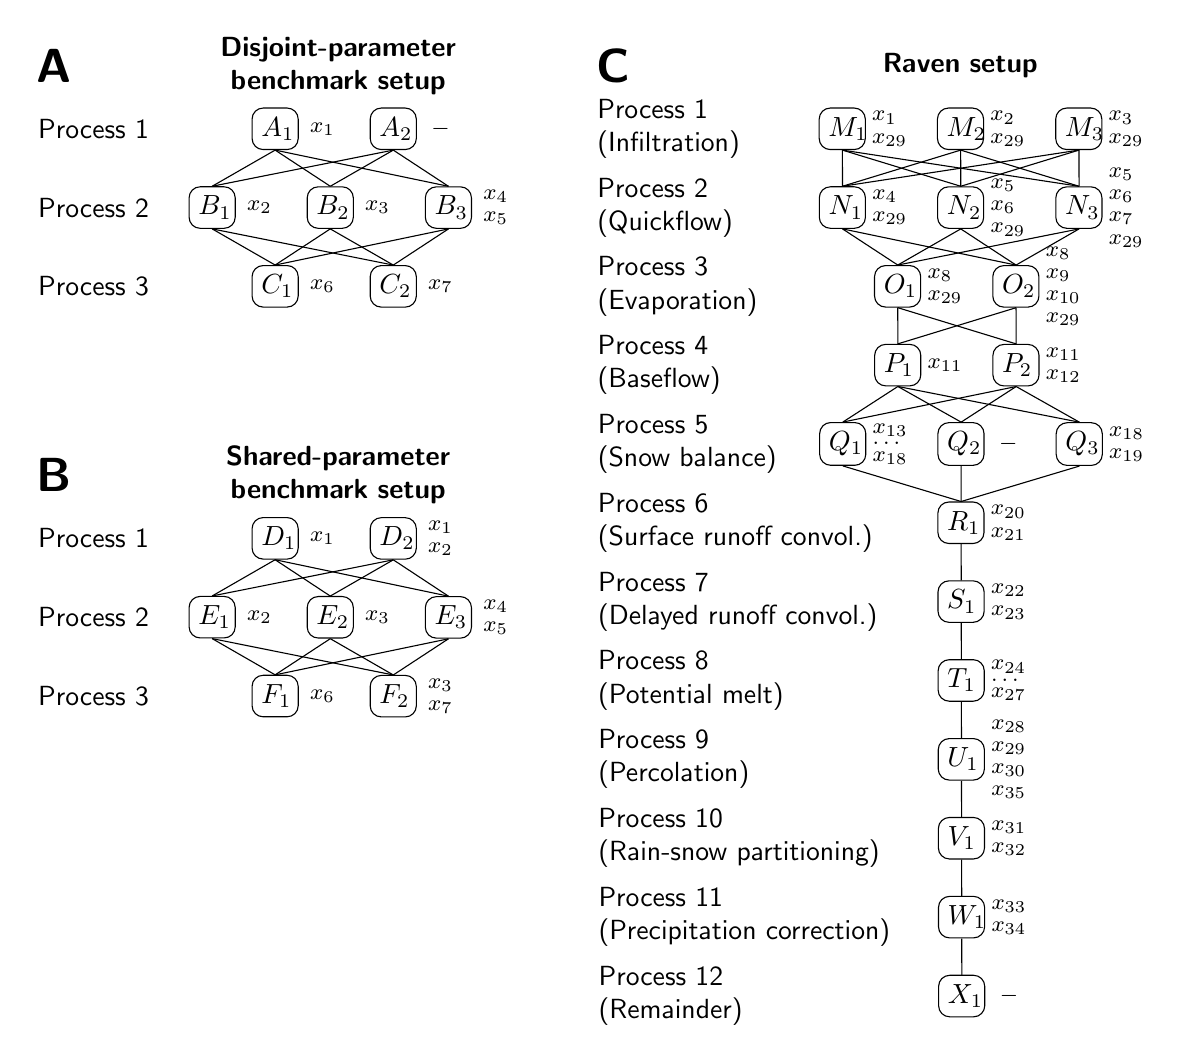
\begin{tikzpicture}[scale=2.5]
		\tikzstyle{block} = [rectangle, draw, fill=white!20, 
		text width=1em, text centered, rounded corners, minimum height=1em]
		\tikzstyle{noblock} = [rectangle, fill=white!20, 
		text width=12em, rounded corners, minimum height=1em]
		\tikzstyle{abcblock} = [rectangle, fill=white!20, 
		text width=1em, rounded corners, minimum height=1em]
		\tikzstyle{line} = [draw, -latex']
		
		% process names :: benchmark setup (=simple setup)
		\node [noblock,align=left] (A) {Process 1};
		\node [noblock,align=left,below of=A] (B) {Process 2};
		\node [noblock,align=left,below of=B] (C) {Process 3};
		
		% process options (simple setup)
		\node [block, node distance=1.5cm,right of=A, xshift=-0.6cm] (a1) {$A_1$};
		\node [block, node distance=1.5cm,right of=a1] (a2) {$A_2$};
		\node [block, node distance=1.5cm,right of=B, xshift=-1.4cm] (b1) {$B_1$};
		\node [block, node distance=1.5cm,right of=b1] (b2) {$B_2$};
		\node [block, node distance=1.5cm,right of=b2] (b3) {$B_3$};
		\node [block, node distance=1.5cm,right of=C, xshift=-0.6cm] (c1) {$C_1$};
		\node [block, node distance=1.5cm,right of=c1] (c2) {$C_2$};
	
		% process names :: benchmark setup (=realistic setup)
		\node [noblock,align=left,below of=A, yshift=-4.2cm] (D) {Process 1};
		\node [noblock,align=left,below of=D] (E) {Process 2};
		\node [noblock,align=left,below of=E] (F) {Process 3};
		
		% process options (realistic setup)
		\node [block, node distance=1.5cm,right of=D, xshift=-0.6cm] (d1) {$D_1$};
		\node [block, node distance=1.5cm,right of=d1] (d2) {$D_2$};
		\node [block, node distance=1.5cm,right of=E, xshift=-1.4cm] (e1) {$E_1$};
		\node [block, node distance=1.5cm,right of=e1] (e2) {$E_2$};
		\node [block, node distance=1.5cm,right of=e2] (e3) {$E_3$};
		\node [block, node distance=1.5cm,right of=F, xshift=-0.6cm] (f1) {$F_1$};
		\node [block, node distance=1.5cm,right of=f1] (f2) {$F_2$};
		
		% process names :: Raven setup
		\node [noblock,align=left,node distance=1.5cm,right of=a2, xshift=3.2cm] (M) {Process 1\\ (Infiltration)};
		\node [noblock,align=left,below of=M] (N) {Process 2\\ (Quickflow)};
		\node [noblock,align=left,below of=N] (O) {Process 3\\ (Evaporation)};
		\node [noblock,align=left,below of=O] (P) {Process 4\\ (Baseflow)};
		\node [noblock,align=left,below of=P] (Q) {Process 5\\ (Snow balance)};
		\node [noblock,align=left,below of=Q] (R) {Process 6\\ (Surface runoff convol.)};
		\node [noblock,align=left,below of=R] (S) {Process 7\\ (Delayed runoff convol.)};
		\node [noblock,align=left,below of=S] (T) {Process 8\\ (Potential melt)};
		\node [noblock,align=left,below of=T] (U) {Process 9\\ (Percolation)};
		\node [noblock,align=left,below of=U] (V) {Process 10\\ (Rain-snow partitioning)};
		\node [noblock,align=left,below of=V] (W) {Process 11\\ (Precipitation correction)};
		\node [noblock,align=left,below of=W] (X) {Process 12\\ (Remainder)};
		
		% process options (Raven setup)
		\node [block, node distance=1.5cm,right of=M, xshift=-0.5cm] (m1) {$M_1$};
		\node [block, node distance=1.5cm,right of=m1] (m2) {$M_2$};
		\node [block, node distance=1.5cm,right of=m2] (m3) {$M_3$};
		\node [block, node distance=1.5cm,right of=N, xshift=-0.5cm] (n1) {$N_1$};
		\node [block, node distance=1.5cm,right of=n1] (n2) {$N_2$};
		\node [block, node distance=1.5cm,right of=n2] (n3) {$N_3$};
		\node [block, node distance=1.5cm,right of=O, xshift=0.2cm] (o1) {$O_1$};
		\node [block, node distance=1.5cm,right of=o1] (o2) {$O_2$};
		\node [block, node distance=1.5cm,right of=P, xshift=0.2cm] (p1) {$P_1$};
		\node [block, node distance=1.5cm,right of=p1] (p2) {$P_2$};
		\node [block, node distance=1.5cm,right of=Q, xshift=-0.5cm] (q1) {$Q_1$};
		\node [block, node distance=1.5cm,right of=q1] (q2) {$Q_2$};
		\node [block, node distance=1.5cm,right of=q2] (q3) {$Q_3$};
		%\node [block, node distance=1.5cm,right of=q3] (q4) {$Q_4$};
		\node [block, node distance=1.5cm,right of=R, xshift=1.0cm] (r1) {$R_1$};
		\node [block, node distance=1.5cm,right of=S, xshift=1.0cm] (s1) {$S_1$};
		\node [block, node distance=1.5cm,right of=T, xshift=1.0cm] (t1) {$T_1$};
		\node [block, node distance=1.5cm,right of=U, xshift=1.0cm] (u1) {$U_1$};
		\node [block, node distance=1.5cm,right of=V, xshift=1.0cm] (v1) {$V_1$};
		\node [block, node distance=1.5cm,right of=W, xshift=1.0cm] (w1) {$W_1$};
		\node [block, node distance=1.5cm,right of=X, xshift=1.0cm] (x1) {$X_1$};
		
		% parameters (simple setup)
		\node [align=left, right of=a1, xshift=-0.4cm] {\footnotesize $x_1$};
		\node [align=left, right of=a2, xshift=-0.4cm] {\footnotesize $-$};
		\node [align=left, right of=b1, xshift=-0.4cm] {\footnotesize $x_2$};
		\node [align=left, right of=b2, xshift=-0.4cm] {\footnotesize $x_3$};
		\node [align=left, right of=b3, xshift=-0.4cm] {\footnotesize $x_4$\\[-4pt]\footnotesize $x_5$};
		\node [align=left, right of=c1, xshift=-0.4cm] {\footnotesize $x_6$};
		\node [align=left, right of=c2, xshift=-0.4cm] {\footnotesize $x_7$};
		
		% parameters (realistic setup)
		\node [align=left, right of=d1, xshift=-0.4cm] {\footnotesize $x_1$};
		\node [align=left, right of=d2, xshift=-0.4cm] {\footnotesize $x_1$\\[-4pt]\footnotesize $x_2$};
		\node [align=left, right of=e1, xshift=-0.4cm] {\footnotesize $x_2$};
		\node [align=left, right of=e2, xshift=-0.4cm] {\footnotesize $x_3$};
		\node [align=left, right of=e3, xshift=-0.4cm] {\footnotesize $x_4$\\[-4pt]\footnotesize $x_5$};
		\node [align=left, right of=f1, xshift=-0.4cm] {\footnotesize $x_6$};
		\node [align=left, right of=f2, xshift=-0.4cm] {\footnotesize $x_3$\\[-4pt]\footnotesize $x_7$};
		
		% parameters (Raven setup)
		\node [align=left, right of=m1, xshift=-0.4cm] {\footnotesize $x_{1}$\\[-4pt]\footnotesize $x_{29}$};
		\node [align=left, right of=m2, xshift=-0.4cm] {\footnotesize $x_{2}$\\[-4pt]\footnotesize $x_{29}$};
		\node [align=left, right of=m3, xshift=-0.4cm] {\footnotesize $x_{3}$\\[-4pt]\footnotesize $x_{29}$};
		\node [align=left, right of=n1, xshift=-0.4cm] {\footnotesize $x_{4}$\\[-4pt]\footnotesize $x_{29}$};
		\node [align=left, right of=n2, xshift=-0.4cm] {\footnotesize $x_{5}$\\[-4pt]\footnotesize $x_{6}$\\[-4pt]\footnotesize $x_{29}$};
		\node [align=left, right of=n3, xshift=-0.4cm] {\footnotesize $x_{5}$\\[-4pt]\footnotesize $x_{6}$\\[-4pt]\footnotesize $x_{7}$\\[-4pt]\footnotesize $x_{29}$};
		\node [align=left, right of=o1, xshift=-0.4cm] {\footnotesize $x_{8}$\\[-4pt]\footnotesize $x_{29}$};
		\node [align=left, right of=o2, xshift=-0.4cm] {\footnotesize $x_{8}$\\[-4pt]\footnotesize $x_{9}$\\[-4pt]\footnotesize $x_{10}$\\[-4pt]\footnotesize $x_{29}$};
		\node [align=left, right of=p1, xshift=-0.4cm] {\footnotesize $x_{11}$};
		\node [align=left, right of=p2, xshift=-0.4cm] {\footnotesize $x_{11}$\\[-4pt]\footnotesize $x_{12}$};
		
		\node [align=left, right of=q1, xshift=-0.4cm] {\footnotesize $x_{13}$\\[-8pt]\footnotesize $\ldots$\\[-6pt]\footnotesize $x_{18}$};
		\node [align=left, right of=q2, xshift=-0.4cm] {\footnotesize $-$};
		\node [align=left, right of=q3, xshift=-0.4cm] {\footnotesize $x_{18}$\\[-4pt]\footnotesize $x_{19}$};
		%\node [align=left, right of=q4, xshift=-0.4cm] {\footnotesize $x_{18}$\\[-4pt]\footnotesize $x_{19}$\\[-4pt]\footnotesize $x_{20}$};
		
		\node [align=left, right of=r1, xshift=-0.4cm] {\footnotesize $x_{20}$\\[-4pt]\footnotesize $x_{21}$};
		
		\node [align=left, right of=s1, xshift=-0.4cm] {\footnotesize $x_{22}$\\[-4pt]\footnotesize $x_{23}$};
		
		\node [align=left, right of=t1, xshift=-0.4cm] {\footnotesize $x_{24}$\\[-8pt]\footnotesize $\ldots$\\[-6pt]\footnotesize $x_{27}$};
		
		\node [align=left, right of=u1, xshift=-0.4cm] {\footnotesize $x_{28}$\\[-4pt]\footnotesize $x_{29}$\\[-4pt]\footnotesize $x_{30}$\\[-4pt]\footnotesize $x_{35}$};
		
		\node [align=left, right of=v1, xshift=-0.4cm] {\footnotesize $x_{31}$\\[-4pt]\footnotesize $x_{32}$};
		
		\node [align=left, right of=w1, xshift=-0.4cm] {\footnotesize $x_{33}$\\[-4pt]\footnotesize $x_{34}$};
		\node [align=left, right of=x1, xshift=-0.4cm] {\footnotesize $-$};
		
		% lines A-B (simple setup)
		\draw (a1.south) -- (b1.north);
		\draw (a1.south) -- (b2.north);
		\draw (a1.south) -- (b3.north);
		\draw (a2.south) -- (b1.north);
		\draw (a2.south) -- (b2.north);
		\draw (a2.south) -- (b3.north);
		
		% lines B-C (simple setup)
		\draw (b1.south) -- (c1.north);
		\draw (b1.south) -- (c2.north);
		\draw (b2.south) -- (c1.north);
		\draw (b2.south) -- (c2.north);
		\draw (b3.south) -- (c1.north);
		\draw (b3.south) -- (c2.north);
		
		% lines D-E (realistic setup)
		\draw (d1.south) -- (e1.north);
		\draw (d1.south) -- (e2.north);
		\draw (d1.south) -- (e3.north);
		\draw (d2.south) -- (e1.north);
		\draw (d2.south) -- (e2.north);
		\draw (d2.south) -- (e3.north);
		
		% lines E-F (realistic setup)
		\draw (e1.south) -- (f1.north);
		\draw (e1.south) -- (f2.north);
		\draw (e2.south) -- (f1.north);
		\draw (e2.south) -- (f2.north);
		\draw (e3.south) -- (f1.north);
		\draw (e3.south) -- (f2.north);
		
		% lines M-N (Raven setup)
		\draw (m1.south) -- (n1.north);
		\draw (m1.south) -- (n2.north);
		\draw (m1.south) -- (n3.north);
		\draw (m2.south) -- (n1.north);
		\draw (m2.south) -- (n2.north);
		\draw (m2.south) -- (n3.north);
		\draw (m3.south) -- (n1.north);
		\draw (m3.south) -- (n2.north);
		\draw (m3.south) -- (n3.north);
		
		% lines N-O (Raven setup)
		\draw (n1.south) -- (o1.north);
		\draw (n1.south) -- (o2.north);
		\draw (n2.south) -- (o1.north);
		\draw (n2.south) -- (o2.north);
		\draw (n3.south) -- (o1.north);
		\draw (n3.south) -- (o2.north);
		
		% lines O-P (Raven setup)
		\draw (o1.south) -- (p1.north);
		\draw (o1.south) -- (p2.north);
		\draw (o2.south) -- (p1.north);
		\draw (o2.south) -- (p2.north);
		
		% lines P-Q (Raven setup)
		\draw (p1.south) -- (q1.north);
		\draw (p1.south) -- (q2.north);
		\draw (p1.south) -- (q3.north);
		%\draw (p1.south) -- (q4.north);
		\draw (p2.south) -- (q1.north);
		\draw (p2.south) -- (q2.north);
		\draw (p2.south) -- (q3.north);
		%\draw (p2.south) -- (q4.north);
		
		% lines Q-R (Raven setup)
		\draw (q1.south) -- (r1.north);
		\draw (q2.south) -- (r1.north);
		\draw (q3.south) -- (r1.north);
		%\draw (q4.south) -- (r1.north);
		
		% lines R-S-T-U-V-W (Raven setup)
		\draw (r1.south) -- (s1.north);
		\draw (s1.south) -- (t1.north);
		\draw (t1.south) -- (u1.north);
		\draw (u1.south) -- (v1.north);
		\draw (v1.south) -- (w1.north);
		\draw (w1.south) -- (x1.north);
		
		% caption
		\node [noblock,align=center,above of=A,xshift=1.7cm,yshift=-0.2cm] {\textbf{Disjoint-parameter benchmark setup}};
		\node [noblock,align=center,above of=D,xshift=1.7cm,yshift=-0.2cm] {\textbf{Shared-parameter benchmark setup}};
		\node [noblock,align=center,above of=A,xshift=9.6cm,yshift=-0.2cm] {\textbf{Raven setup}};
		
		% ABC
		\node [abcblock,align=center,above of=A,xshift=-1.95cm,yshift=-0.2cm] {{\LARGE \textbf{A}}};
		\node [abcblock,align=center,above of=D,xshift=-1.95cm,yshift=-0.2cm] {{\LARGE \textbf{B}}};
		\node [abcblock,align=center,above of=M,xshift=-1.95cm,yshift=-0.2cm] {{\LARGE \textbf{C}}};
		
	\end{tikzpicture}

\end{document}



